
\section{Profiling Results}
% Should include figures for initial implementation and the final implementation(Test id 15)
\subsection{Number of calls}
From \figureref{fig:ncc} we can see that the most called function, a lambda in the SURFExtractor module is part of the setup process, meaning the relevant functions are \mono{boltzmannProbs} in the rbm module, the \mono{fuse} function from the cffun module and the \mono{err} function in the learn weights module.


\begin{figure}
    \centering
    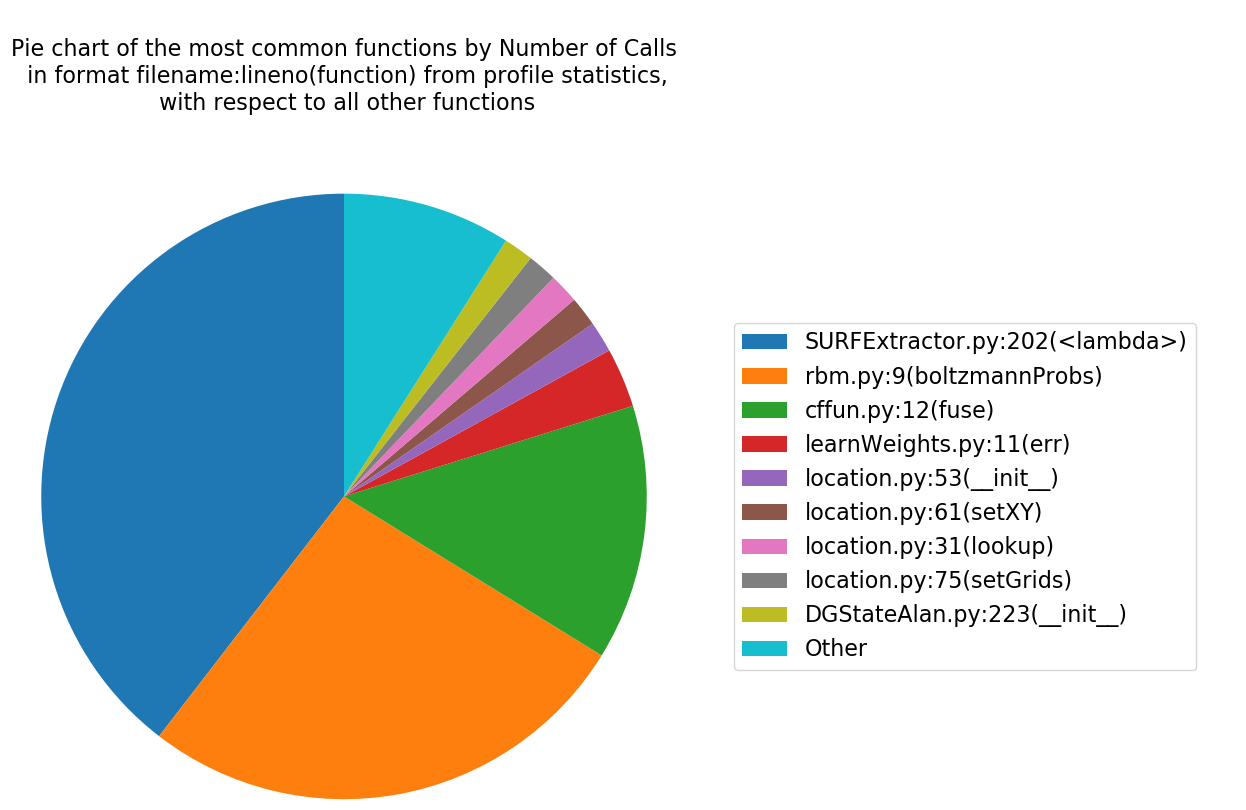
\includegraphics[width=0.7\textwidth]{figures/res_profiling/number_calls_cpu_crop.png}
    \caption{Number of calls for the CPU implementation of the model.}
    \label{fig:ncc}
\end{figure}

\begin{figure}
    \centering
    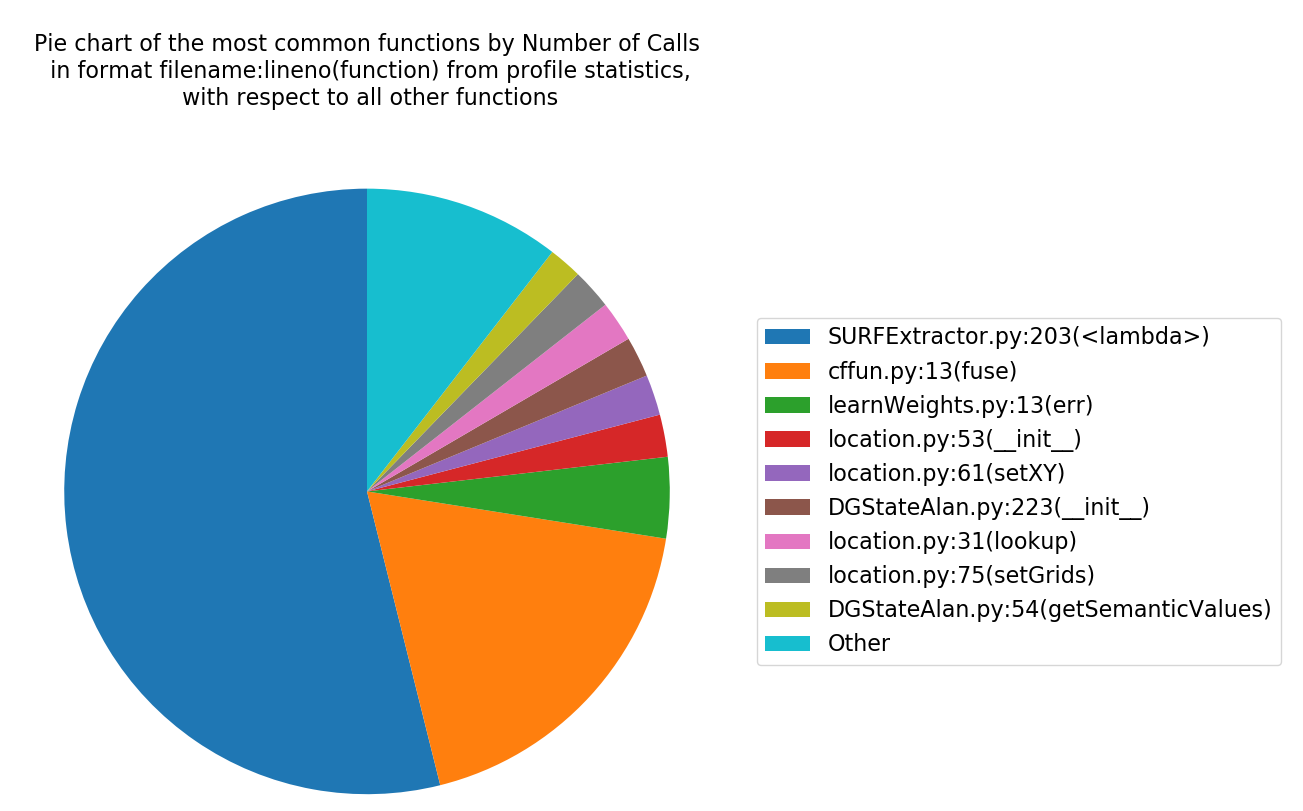
\includegraphics[width=0.7\textwidth]{figures/res_profiling/number_calls_gpu_crop.png}
    \caption{Number of calls for the GPU implementation of the model.}
    \label{fig:ncg}
\end{figure}

In contrast, profiling the Tensorflow version (\figureref{fig:ncg}) shows the lambda function from SURFExtractor taking a larger proportion of the total number of calls.
This is likely due to the usage of the \mono{tf.function} decorator optimisation.
The decorator converts the function into an optimised Tensorflow data call graph, which is loaded into the memory of the GPU at runtime.



Tensorflow processes the calls to the function such that the profiler only records the first time each call to \mono{boltzmannProbs} is hit, as opposed to everytime.
The \mono{cffun\#fuse} function has approximately the same amount of calls, and can probably be reduced by applying the \mono{tf.function} decorator.
Finally the \mono{learnWeights\#err} function has a constant number of calls across both implementations as it is not affected by the randomness of the model.


\subsection{Total time}

The more interesting profiling results come from the total time spent executing the function, excluding calls to other functions.
Initially the main functions that take the most time are the \mono{learn} function of the \mono{learnWeights} module, the \mono{boltzmannProbs} function of the \mono{rbm} module and the \mono{fuse} function of \mono{cffun} module as seen in \figureref{fig:ttc}.

After applying the parallel refactoring, the \mono{learnWeights\#learn} function takes a larger proportion of the overall time taken, as seen in \figureref{fig:ttg}.
The \mono{cffun\#fuse} function also has an increase in the proportion of time taken.
However, given that the overall time taken increases with a small amount of nodes, it indicates that there may be an underlying algorithmic problem which causes this behaviour.

\picturesque{figures/res_profiling/tot_time_cpu_crop.png}{Total time for function calls for the CPU implementation of the model.}{fig:ttc}

\picturesque{figures/res_profiling/tot_time_gpu_crop.png}{Total time for function calls for the GPU implementation of the model.}{fig:ttg}


In addition, the \mono{boltzmannProbs} function appears to have a large reduction in time taken.
However this is likely due to the \mono{tf.function} decorator function mapping the original function to a data call graph that runs purely on the GPU, which the Python profiler does not have access to.
This can be seen when using the line profiler on the \mono{boltzmannProbs} function.

%insert listing or similar thing depicting the output of line profiler, with full excerpt in an appendix.
\coderef{profiling:line_boltzmann} shows the results of profiling the \mono{boltzmannProbs} function line by line. 
It can be seen that the main bottleneck is the multiplication of the inputs and weights, taking approximately 60\% of the overall time.
This is likely due to the asynchronous nature of matrix multiplication, which is applied across a given dimension of the inputs. 


\begin{minipage}{\linewidth}
\begin{lstlisting}[caption=Line by line profiling of the rbm\#boltzmannProbs function in eager execution mode, label=profiling:line_boltzmann]
Total time: 237.186 s
Function: boltzmannProbs at line 9

Line #      Hits         Time  Per Hit   % Time  Line Contents
==============================================================
     9                                           @profile
    10                                           #@tf.function
    11                                           def boltzmannProbs(W, x, axis=0):      # RETURNS THE PROBABILITY OF A NODE BEING ON
    12    252240  143312866.0    568.2     60.4      mult = tf.tensordot(W, x, axis)
    13    252240   12193753.0     48.3      5.1      squeezed = tf.squeeze(mult)
    14    252240    6917896.0     27.4      2.9      E_on  = -squeezed       #penalty is the negative of the reward (just to make it look like energy
    15    252240   20604441.0     81.7      8.7      E_off = 0.0*E_on
    16    252240   13057317.0     51.8      5.5      Q_on = tf.math.exp(-E_on)       #as energy is negated, we have e^(reward)
    17    252240   12601996.0     50.0      5.3      Q_off = tf.math.exp(-E_off)
    18    252240   28258157.0    112.0     11.9      P_on = Q_on / (Q_on + Q_off)
    19    252240     239234.0      0.9      0.1      return P_on
\end{lstlisting}
\end{minipage}



